\documentclass[conference]{IEEEtran}

\usepackage[hyphens]{url}
\usepackage{amsmath}
\usepackage{graphicx}


\title{An Interpretable, Leakage-Aware Baseline for Predicting\\
One-Century Territorial Contraction in Historical Polities}

\author{
\IEEEauthorblockN{Shailesh Mishra (PES2UG24CS453), Shalik S (PES2UG24CS454),\\
Spoorthi A N (PES2UG24CS515), Aaron (PES2UG24CSXXX)}
\IEEEauthorblockA{Department of Computer Science and Engineering\\
PES University, Bengaluru, India}
}

\begin{document}
\maketitle

\begin{abstract}
Predictive models of historical state decline are easy to build and hard to
trust: tiny positive counts, autocorrelated trajectories, and leaky evaluation
routinely produce scores that look better than they are. This paper presents an
interpretable, leakage-aware baseline for predicting whether a historical
polity loses at least 30\% of its recorded territory over the following
100~years, derived from the Equinox release of the Seshat Global History
Databank. The implemented target is a territorial-contraction warning, not a
validated ``civilizational collapse detector.'' After auditing the ingestion of
the AggrSCWarAgriRelig worksheet, only 98 polity-century observations carry an
exactly windowed label: 92 non-contractions and 6 contractions spanning 76
polities, 25 NGAs, and years $-3800$ to $1800$. A class-balanced logistic
regression over seven contemporaneous indicators and their prior-century
differences is evaluated with polity-grouped stratified cross-validation,
repeated seeds, and a chronological holdout whose training window cannot cross
the cutoff. Out-of-fold precision--recall AUC is 0.122 at seed~0 (base rate
0.061), ranges from 0.093 to 0.122 across three seeds, and reaches 0.141 on the
chronological holdout. These results demonstrate evaluation discipline, not
strong predictive performance. The contribution is an end-to-end, reproducible
workflow for operationalizing and auditing historical territorial-contraction
warnings: honest labels, leakage controls, a false-positive review with
coefficient-based case explanations, a curated historical face-validity audit,
label-sensitivity analysis, and an interactive dashboard with reusable exports.
The present evidence is insufficient to claim reliable collapse prediction.
\end{abstract}

\begin{IEEEkeywords}
historical polities, Seshat, Equinox, territorial contraction, leakage-aware
evaluation, interpretable baseline, grouped cross-validation
\end{IEEEkeywords}

\section{Introduction}
Quantitative history increasingly uses machine learning to anticipate state
fragility, but the data regime is unforgiving: outcomes are rare, records are
irregular, and naive pipelines leak information across time and across polity
identity. A model that appears accurate under a random split can fail entirely
once within-polity correlation and future information are controlled.

This paper describes a deliberately conservative baseline system. The goal is
not to present a finished predictor but to build the evaluation and audit
machinery that a trustworthy predictor would require, and to report what the
data can and cannot support. The system operationalizes a specific, checkable
target: given indicators observed at time $t$, warn when a polity will lose at
least 30\% of its recorded territory by $t{+}100$ years. We make the following
contributions:

\begin{itemize}
\item A label-construction audit that converts an informal ``30\% loss'' rule
into an exact log-scale threshold with strictly observed endpoints, yielding
98 labelled polity-century observations.
\item A leakage-aware evaluation protocol: polity-grouped stratified folds with
an explicit no-overlap assertion, fold-local imputation and scaling, repeated
seeds, and a chronological holdout that excludes any training record whose
label window crosses the cutoff year.
\item An audit layer on top of the model: a pre-specified confident
false-positive queue, case-level coefficient explanations (explicitly not
SHAP), a curated historical face-validity review of eleven cases, and a label
sensitivity analysis over pre-specified contraction definitions.
\item A Streamlit dashboard and flat-file exports that make every intermediate
artifact inspectable and reusable.
\end{itemize}

The honest headline is negative and we state it plainly: with six positive
labels, all performance estimates are unstable, and the baseline is not a
deployable collapse predictor.

\section{Data and Label Engineering}
\subsection{Source and ingestion audit}
We use the \emph{AggrSCWarAgriRelig} worksheet of the Equinox release of the
Seshat Global History Databank~\cite{turchin2018,seshat}. The ingestion audit
converts the missing-value sentinel $-999$ to null and removes filler rows in
which the unique identifier equals the row count, reducing 1{,}494 source rows
to 609 retained rows.

\subsection{Label construction}
Historical coverage is irregular, so a usable label requires an \emph{exact}
future observation at $t{+}100$ for the same composite polity identifier
(NGA, PolID); we do not interpolate or fabricate endpoints. Territory
($\mathrm{Terr}$) is recorded on a $\log_{10}$ scale, so a 30\% contraction
over the following century is
\begin{equation}
\mathrm{Terr}_{t+100} - \mathrm{Terr}_{t} \le \log_{10}(0.7) = -0.154902 .
\end{equation}
This corrects the common but incorrect practice of thresholding the log-scaled
difference at $-0.30$, which would correspond to a 50\% loss rather than 30\%.
Retaining only rows with observed territory at both endpoints yields
\textbf{98 labelled polity-century observations}: \textbf{92 non-contractions
and 6 contractions}, covering 76 polities, 25 NGAs, and years $-3800$ to
$1800$. The positive base rate is 0.0612.

\subsection{Territorial contraction is not regime collapse}
Throughout, a ``contraction'' is a measured change in recorded territory. A
polity can remain historically significant while losing territory, and a regime
can collapse without an immediate territorial record of it. The label must not
be read as a collapse detector.

\section{Predictors and Feature Construction}
The baseline uses seven Equinox indicators observed at time $t$: population
(Pop), capital population (Cap), hierarchy (Hier), governance (Gov),
infrastructure (Infra), information systems (Info), and money (Money). Each
indicator enters both contemporaneously and as its prior-century difference,
e.g.\ $\mathrm{Pop}_t - \mathrm{Pop}_{t-100}$, giving 14 candidate inputs.

Missing feature values and missing deltas are never fabricated: median
imputation is fitted \emph{within each training fold} and applied to the
corresponding test fold. Delta coverage is sparse, because many polity
trajectories lack an observation exactly one century earlier; we treat this
sparsity as a first-class limitation rather than imputing it away globally.

\section{Predictive Baseline and Evaluation Protocol}
\subsection{Model}
The model is a class-balanced logistic regression wrapped in a pipeline with
median imputation and standardization. Logistic regression is chosen for
interpretability: every warning can be decomposed into per-feature coefficient
contributions.

\subsection{Grouped, leakage-controlled evaluation}
The main evaluation is five-fold StratifiedGroupKFold grouped by the composite
polity identifier. The code asserts that no polity appears in both the training
and test partitions of any fold, preventing within-polity leakage. All
preprocessing is fitted only on each training partition, and out-of-fold (OOF)
probabilities are generated for every labelled observation. Accuracy is
intentionally not reported: with a 6.1\% positive rate it would be misleading.

\subsection{Main result}
At the default threshold of 0.5, the seed-0 grouped OOF baseline achieves
precision 0.0909, recall 0.5000, and PR-AUC 0.1224, raising 33 warnings: 3 true
positives and 30 false positives (Table~\ref{tab:main},
Fig.~\ref{fig:pr}). These numbers are
descriptive and highly unstable; with six positive labels, moving a single
positive case between folds materially changes every metric.

\begin{table}[t]
\centering
\caption{Seed-0 grouped OOF performance at threshold 0.5}
\label{tab:main}
\begin{tabular}{lc}
\hline\hline
Metric & Value \\
\hline
Precision & 0.0909 \\
Recall & 0.5000 \\
PR-AUC & 0.1224 \\
Positive base rate & 0.0612 \\
Warnings raised & 33 \\
True positives / False positives & 3 / 30 \\
\hline\hline
\end{tabular}
\end{table}

\begin{figure}[t]
\centering
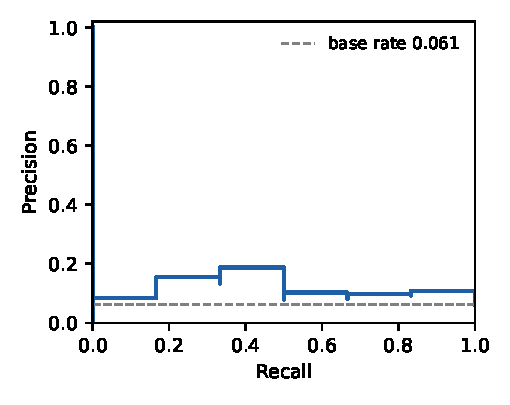
\includegraphics[width=\columnwidth]{fig_pr_curve.pdf}
\caption{Grouped out-of-fold precision--recall curve (seed~0) for the primary
30\% contraction label. Average precision is 0.122 against a 0.061 positive
base rate: a real but weak ranking signal, not a usable warning system.}
\label{fig:pr}
\end{figure}

\section{Leakage and Robustness Checks}
\subsection{Repeated grouped evaluation}
We repeat the grouped evaluation with seeds 0, 1, and 2. PR-AUC ranges from
0.0934 to 0.1224, showing sensitivity to fold allocation; we report the range
rather than the best seed.

\subsection{Chronological holdout}
We implement a chronological holdout with cutoff year 800. Any training record
whose 100-year label window reaches or crosses the cutoff is excluded, so no
future-territory information crosses the temporal boundary. The post-cutoff
test set contains 47 observations with 3 positive cases; it achieves precision
0.1053, recall 0.6667, and PR-AUC 0.1406. These checks demonstrate evaluation
discipline under both identity-based and time-based separation; they do not
rescue predictive performance.

\section{False-Positive Audit and Interpretation}
False-positive cases are selected \emph{before} interpretation using a
pre-specified rule: the 95th percentile of OOF probabilities. Five high-scoring
survival cases are reviewed: Northern Song China at 1000, Roman polity
observations at years 0 and 100, and Ming China at 1400 and 1500
(Fig.~\ref{fig:traj}).

For explanatory analysis only, the logistic model is fitted on the full
dataset, and each feature's standardized coefficient contribution is computed
per case. We stress that these are coefficient contributions, \emph{not} SHAP
values; the long-form export retains the legacy filename
\texttt{shap\_long.csv} for compatibility. The review identifies current
hierarchy, population, information, and capital-related signals as major
contributors in the selected cases. The dashboard keeps manual fields for a
reviewer to classify each case and record historical notes, so the audit is a
workflow, not a one-off table.

\begin{figure*}[t]
\centering
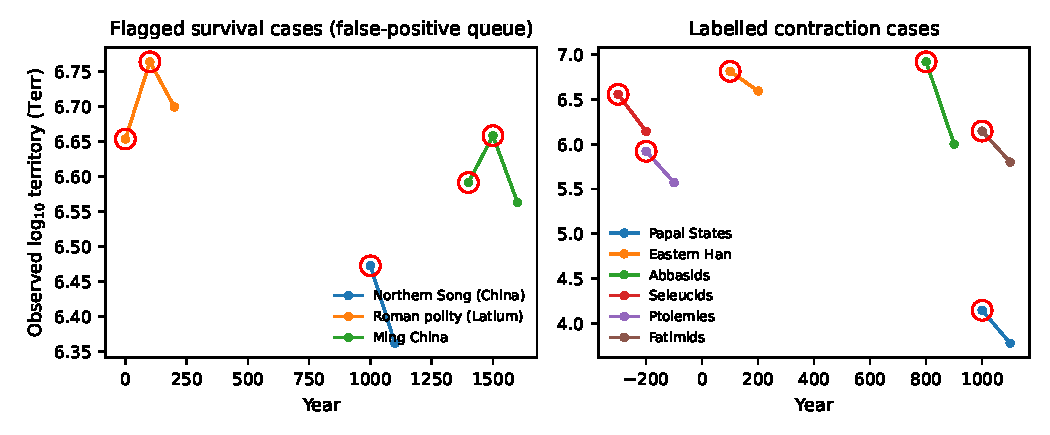
\includegraphics[width=\textwidth]{fig_trajectories.pdf}
\caption{Observed $\log_{10}$ territory trajectories for the audited cases.
Left: the polities behind the five pre-specified high-scoring survival cases
(red circles mark the flagged polity-centuries). Right: the six labelled
contraction cases (red circles mark the century at which the contraction label
applies). Only polity-centuries with an exact next-century endpoint appear;
historical coverage is sparse by construction. Territory is the label source
and is never a model input.}
\label{fig:traj}
\end{figure*}

\section{Historical Face-Validity Audit}
Beyond the false-positive queue, we conduct a curated review of 11 historically
contextualized cases: the five false alarms plus all six labelled territorial
contractions. Each record contains the polity, time, observed territory
transition, $\log_{10}$ change, area ratio, source URL, and an interpretation
note. The contraction cases are the Papal States, Eastern Han, the Abbasids,
the Seleucids, the Ptolemies, and the Fatimids. No label corrections resulted:
\texttt{verified\_correction = none} for every audit record. The audit's value
is procedural: it forces each confident warning and each label to survive
contact with the historical record.

\section{Label Sensitivity Analysis}
The choice of contraction threshold is a modelling decision, so we test
pre-specified alternatives and report all of them (Table~\ref{tab:sens}): a
20\% loss rule (9 positives; grouped PR-AUC 0.2532, leave-polity-out 0.2314),
the primary 30\% rule (6 positives; 0.1224, 0.1008), and a 50\% rule
(5 positives; 0.1040, 0.0818). This is a sensitivity analysis, not a
threshold-selection exercise: the study does not adopt a definition because it
produces better numbers.

\begin{table}[t]
\centering
\caption{Pre-specified label sensitivity (PR-AUC)}
\label{tab:sens}
\begin{tabular}{lccc}
\hline\hline
Loss rule & Positives & Grouped & Leave-polity-out \\
\hline
20\% & 9 & 0.2532 & 0.2314 \\
30\% (primary) & 6 & 0.1224 & 0.1008 \\
50\% & 5 & 0.1040 & 0.0818 \\
\hline\hline
\end{tabular}
\end{table}

\begin{figure}[t]
\centering
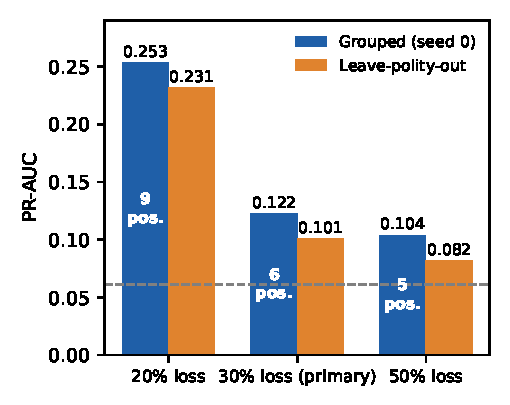
\includegraphics[width=\columnwidth]{fig_label_sensitivity.pdf}
\caption{Pre-specified label sensitivity: grouped (seed~0) and
leave-polity-out PR-AUC for three contraction definitions, with positive
counts; the dashed line marks the primary 6.1\% base rate. This is a sensitivity
analysis, not a threshold-selection exercise;
the study does not adopt a definition because it produces better numbers.}
\label{fig:sens}
\end{figure}

\section{Model-Variant Experiments}
We compare the seven-input and fourteen-input variants under a
Leave-One-Polity-Out outer evaluation. In practice the two coincide here: the
training-fold missingness filter removes every prior-century-difference input
(each is missing on more than 60\% of training rows), so all fits reduce to
the seven contemporaneous indicators. Tuned variants select the logistic
regularization strength $C \in \{0.01, 0.1, 1, 10\}$ by grouped validation
inside each outer training partition. The untuned variant reaches PR-AUC
0.1008; tuning improves this to 0.1278, still far too weak and data-limited to
support deployment claims. At a 0.7 warning threshold the untuned variant
raises eighteen warnings, catching two true contractions with sixteen false
warnings, while the tuned variant raises none. We present this as an
operating-point trade-off, not as a model improvement: threshold changes
redistribute errors rather than remove them.

\section{Interactive Dashboard and Reusable Exports}
A Streamlit dashboard exposes the pipeline to inspection:
\begin{enumerate}
\item a polity browser with century-by-century plots of the seven current
indicators;
\item a false-positive explorer showing ranked feature differences, case-level
coefficient contributions, OOF risk, and manual-review metadata;
\item a what-if interface in which a user adjusts all 14 model inputs and
receives an illustrative predicted probability, clearly labelled as non-causal
and illustrative.
\end{enumerate}

\begin{figure}[t]
\centering
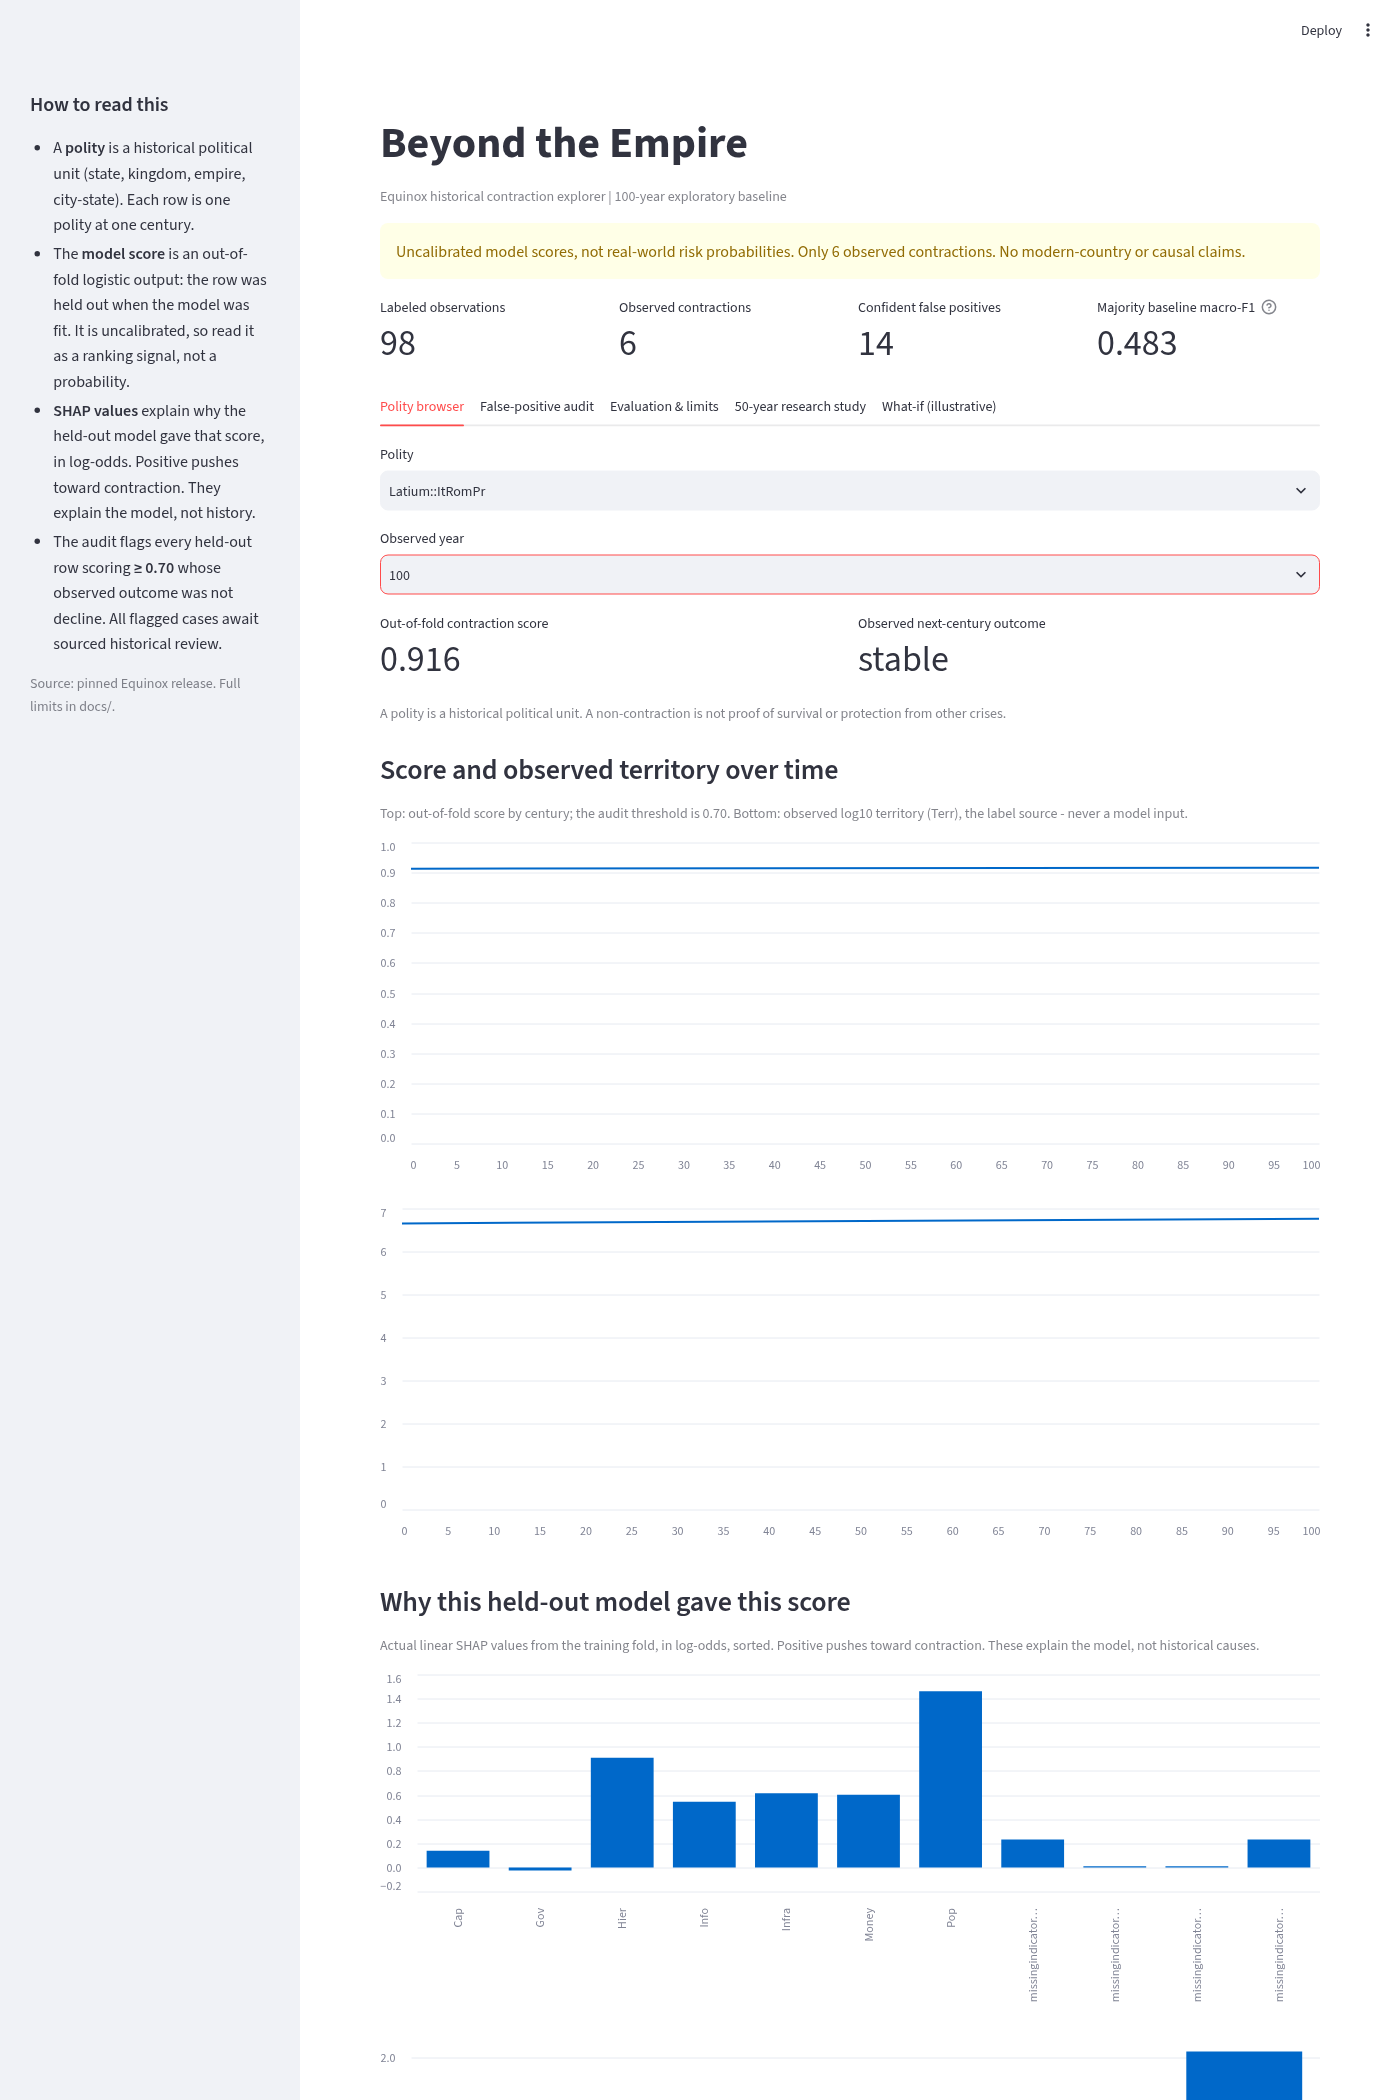
\includegraphics[width=\columnwidth]{fig_dashboard_browser.png}
\caption{Dashboard polity browser for Latium::ItRomPr at year 100, a flagged
survival case: out-of-fold score and observed outcome, score and observed
territory over time, and per-case feature-contribution bars from the held-out
fold. Scores are uncalibrated ranking signals.}
\label{fig:dash-browser}
\end{figure}

\begin{figure}[t]
\centering
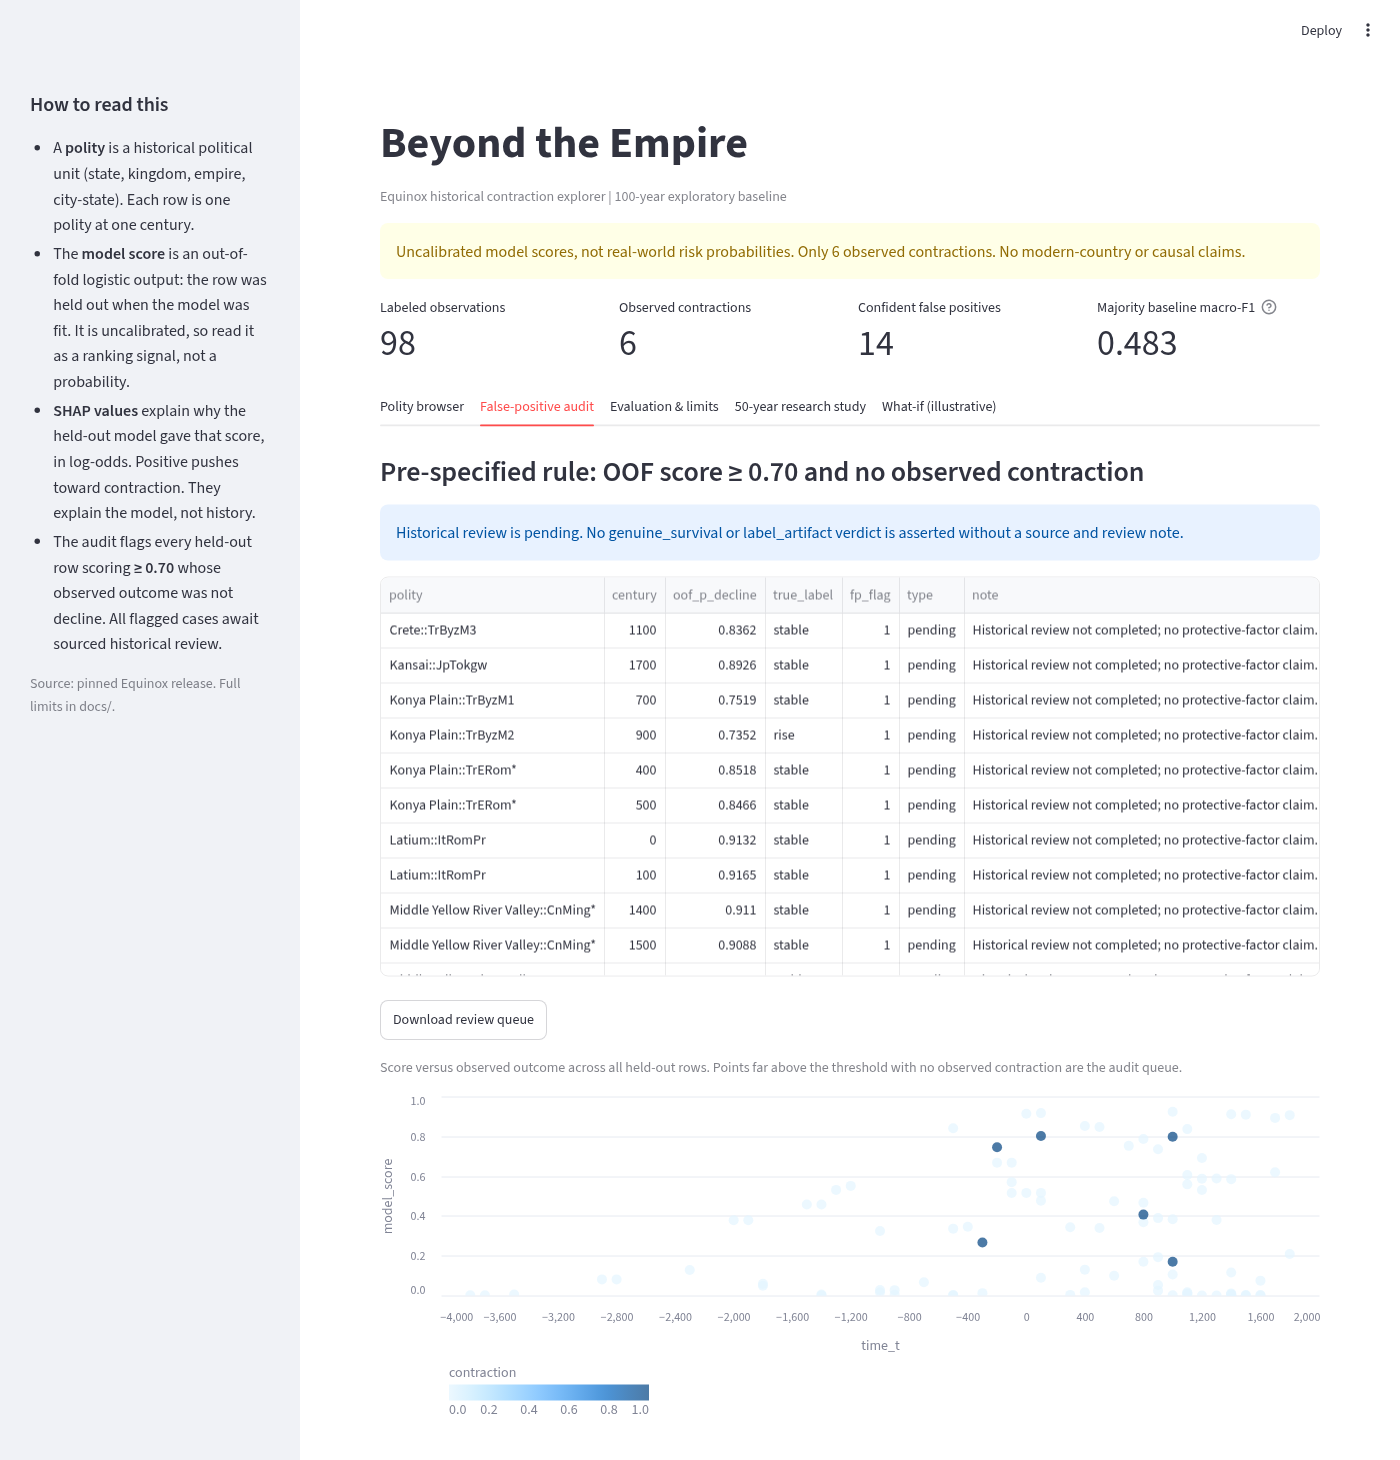
\includegraphics[width=\columnwidth]{fig_dashboard_fpexplorer.png}
\caption{Dashboard false-positive explorer. The pre-specified audit rule
(out-of-fold score $\geq 0.70$ with no observed contraction) flags fourteen
polity-centuries, each awaiting sourced historical review; the scatter shows
score versus observed outcome across all held-out rows.}
\label{fig:dash-fp}
\end{figure}

\begin{figure}[t]
\centering
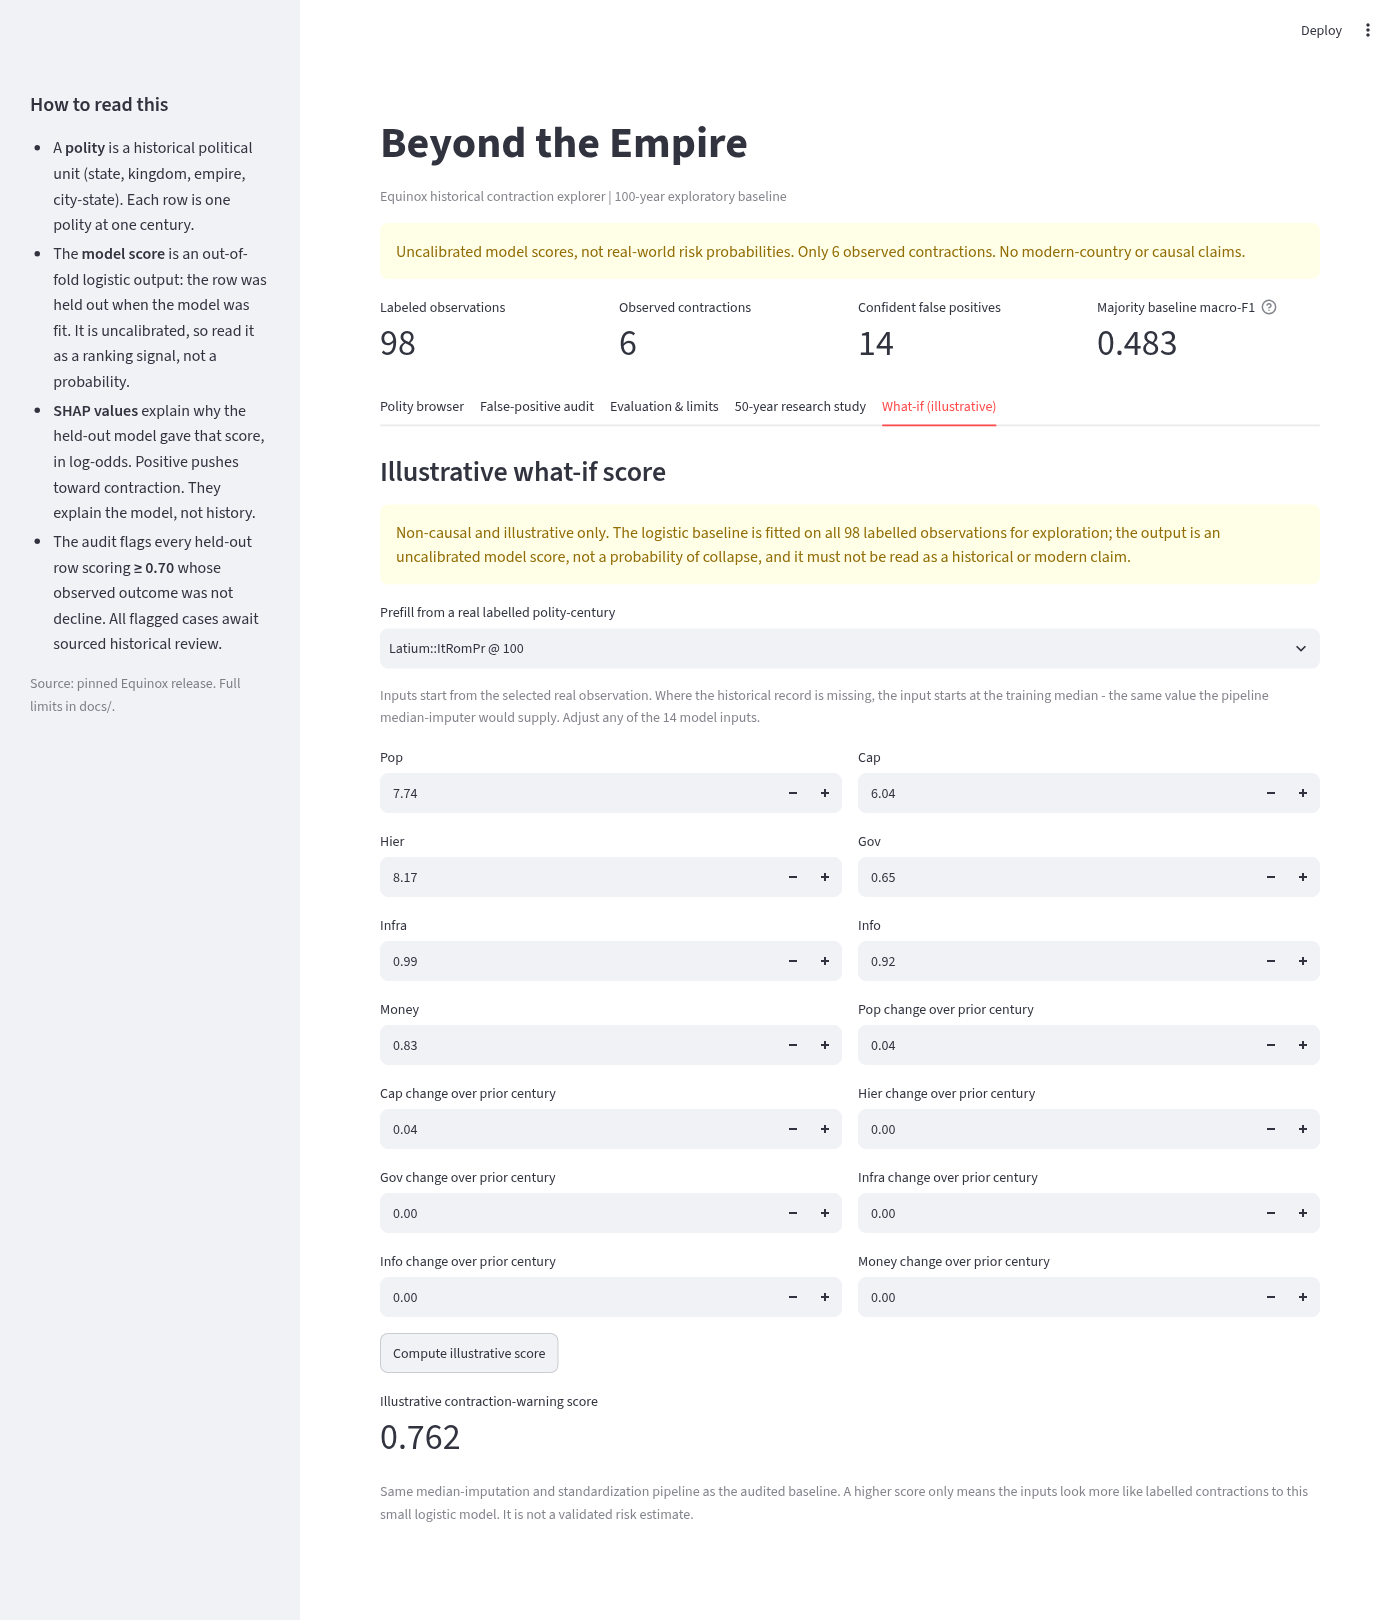
\includegraphics[width=\columnwidth]{fig_dashboard_whatif.png}
\caption{Dashboard what-if interface, prefilled from a real labelled
polity-century. Adjusting any of the 14 model inputs produces an illustrative
score through the same imputation and scaling pipeline; the output is
non-causal, uncalibrated, and not a validated risk estimate.}
\label{fig:dash-whatif}
\end{figure}

Figures~\ref{fig:dash-browser}--\ref{fig:dash-whatif} show the three audit
surfaces.
Separate flat-file exports support downstream visualization:
\texttt{predictions.csv} (one OOF prediction per labelled polity-century),
\texttt{shap\_long.csv} (long-form coefficient contributions despite its legacy
filename), and \texttt{fp\_cases.csv} (review cases). All exports use polity
and observed century/time as join keys. A companion Power BI report renders the
same exports for presentation.

\section{Limitations}
This project is an auditable baseline, not a finished predictive system. The
central limitations are: only six positive outcomes; sparse lagged features
from irregular historical sampling; uncertain historical territorial
boundaries; no external validation set; no comparison against crisis records
such as CrisisDB yet; and no causal interpretation of any coefficient or
dashboard output.

\section{Conclusion and Future Work}
We built an end-to-end, reproducible workflow for operationalizing and auditing
historical territorial-contraction warnings: exact-window labels on a corrected
log-scale threshold, grouped and chronological leakage controls, a
pre-specified false-positive queue with coefficient-based explanations, a
curated historical face-validity audit, label sensitivity analysis, and
inspectable exports. The present evidence is insufficient to claim reliable
collapse prediction, and the system is designed so that stronger claims cannot
be smuggled in later. Future work is to improve outcome data, validate the
operational label against crisis records, investigate the false alarms
historically, and evaluate on genuinely unseen historical cases.

\begin{thebibliography}{9}
\bibitem{turchin2018}
P.~Turchin et al., ``Quantitative historical analysis uncovers a single
dimension of complexity that structures global variation in human social
organization,'' \emph{Proc. Natl. Acad. Sci. USA}, vol.~115, no.~2,
pp.~E144--E151, 2018.
\bibitem{seshat}
Seshat: Global History Databank, Equinox release, AggrSCWarAgriRelig
worksheet. [Online]. Available: \url{https://seshatdatabank.info}
\bibitem{sklearn}
F.~Pedregosa et al., ``Scikit-learn: Machine learning in Python,''
\emph{J. Mach. Learn. Res.}, vol.~12, pp.~2825--2830, 2011.
\end{thebibliography}

\end{document}
